\newpage

\subsection{Neuroevolution of Augmenting Topologies}
Neuroevolution uses evolutionary algorithms, such as genetic algorithms, to optimise ANNs \cite{neuroevolution_review}.
One such algorithm is Neuroevolution of Augmenting Topologies (NEAT), which evolves the topology and weights of ANNs \cite{neat_main, neat_short, neat_phd}.
It gained traction when published since it adressed some previous problems in neuroevolution and illustrated how the structure of ANNs could be
evolved as to increase the learning speed. Other versions of NEAT have been developed since which can evolve ANNs of larger scale and complexity more efficiently.

NEAT uses a direct encoding; genomes contain connection and node genes which specify the network (see Figure \ref{mapping}). Each connection gene is identified
by a number and references the two node genes it spans. The node gene is also identified by a number.

\begin{figure}[htb]
    \begin{mdframed}
        \begin{subfigure}[b]{0.45\textwidth}
            \centering
            \resizebox{1\textwidth}{!}{\input{resources/tex/genotype.tex}}
            \caption{Genotype.}
            \label{genotype}
        \end{subfigure}
        \begin{subfigure}[b]{0.45\textwidth}
            \centering
            \resizebox{0.65\textwidth}{!}{\input{resources/tex/phenotype.tex}}
            \caption{Phenotype.}
            \label{phenotype}
        \end{subfigure}
    \end{mdframed}
    \caption{Example of a genome and its corresponding ANN phenotype.}
    \label{mapping}
\end{figure}


The initial population of genomes consists of structurally identical and fully connected networks without any hidden nodes.
New structures emerge through structural mutations which can add new node or connection genes to the genomes. Nodes are added by splitting an existing
connection, which is disabled and two new connection genes are added along with the new node gene (see Figure \ref{node_mutation}).

\begin{figure}[htb]
    \begin{mdframed}
        \begin{subfigure}[b]{0.45\textwidth}
            \centering
            \resizebox{1\textwidth}{!}{\setlength{\arrayrulewidth}{0.01mm}
\setlength{\tabcolsep}{5pt}
\renewcommand{\arraystretch}{1}

\arrayrulecolor[HTML]{000000}

\vspace{0.2cm}
\begin{tabular}{ |p{0.5cm}|p{1.8cm}|  }
    \hline
    \rowcolor{lightgray} \multicolumn{2}{|c|}{Node genes} \\
    \hline
    Id & Type \\
    \hline
    1 & \cellcolor{green!50} INPUT \\
    \hline
    2 & \cellcolor{green!50} INPUT \\
    \hline
    3 & \cellcolor{red!50} OUTPUT \\
    \hline
    4 & \cellcolor{blue!50} HIDDEN \\
    \hline
\end{tabular}

\begin{tabular}{ |p{0.5cm}|p{0.5cm}|p{0.7cm}|p{1.2cm}|p{1.4cm}|  }
    \hline
    \rowcolor{lightgray} \multicolumn{5}{|c|}{Connection genes} \\
    \hline
    Id & In & Out & Weight & Enabled \\
    \hline
    1 & \cellcolor{green!50} 1 & \cellcolor{red!50} 3 & 0.3 & True \\
    2 & \cellcolor{green!50} 2 & \cellcolor{red!50} 3 & 0.5 & False \\
    3 & \cellcolor{green!50} 2 & \cellcolor{blue!50} 4 & 1 & True \\
    4 & \cellcolor{blue!50} 4 & \cellcolor{red!50} 3 & 0.5 & True \\
    \hline
\end{tabular}
}
            \caption{Genotype.}
            \label{node_genotype}
        \end{subfigure}
        \begin{subfigure}[b]{0.45\textwidth}
            \centering
            \resizebox{0.65\textwidth}{!}{\input{resources/tex/added_node_phenotype.tex}}
            \caption{Phenotype.}
            \label{node_phenotype}
        \end{subfigure}
    \end{mdframed}
    \caption{Example of a node mutation.}
    \label{node_mutation}
\end{figure}


Mutations can also add new connections, which span any two previously unconnected nodes (see Figure \ref{link_mutation}).
Connections can be of three types, depending on their output node. Loops are connections that start and end on the same node. Recurrent connections go backwards in the network to a node closer to an
input node. Finally, forward connections end on a node closer to an output node. The first two types of connections can provide a form of short term memory by repeating
signals from a previous time step.

\begin{figure}[htb]
    \begin{mdframed}
        \begin{subfigure}[b]{0.45\textwidth}
            \centering
            \resizebox{1\textwidth}{!}{\input{resources/tex/added_link_genotype.tex}}
            \caption{Genotype.}
            \label{link_genotype}
        \end{subfigure}
        \begin{subfigure}[b]{0.45\textwidth}
            \centering
            \resizebox{0.65\textwidth}{!}{\input{resources/tex/added_link_phenotype.tex}}
            \caption{Phenotype.}
            \label{link_phenotype}
        \end{subfigure}
    \end{mdframed}
    \caption{Example of a link mutation of the genotype from Figure \ref{node_genotype}.}
    \label{link_mutation}
\end{figure}


New structures can also be created during crossover, in which the genes of two genomes are combined.
The id attribute of the genes, referred to as an innovation number, serves to uniquely identify each mutation that has occured.
Each time a new link or node is added, a database containing all previous mutations and their ids is referenced.
As such, identical mutations are labeled with the same id.
These numbers are used during speciation and crossover. NEAT divides the population of genomes into species based on their structural
similarity, which is measured as a compatibility score.


\todo{Explain speciation and fitness sharing}

\begin{figure}[htb]
    \begin{mdframed}
    \begin{tikzpicture}

        \begin{scope}
            \tikzstyle{box} = [rectangle, rounded corners, minimum width=3.8cm, minimum height=1.6cm,text centered, draw=black, fill=white]

% Population
\node [box] (population) {};
\node [anchor=north] at (population.north) {Population};

\node (line1) [anchor=south west] at (population.south west) {$\coloredrule{10mm}{1mm}{green}$};
\node (line2) [anchor=south west] at (line1.south east) {$\coloredrule{10mm}{1mm}{Salmon}$};
\node (line3) [anchor=south west] at (line2.south east) {$\coloredrule{10mm}{1mm}{Periwinkle}$};
\node (line4) [anchor=south west] at (line1.north west) {$\coloredrule{10mm}{1mm}{red}$};
\node (line5) [anchor=south west] at (line2.north west) {$\coloredrule{10mm}{1mm}{SeaGreen}$};
\node (line6) [anchor=south west] at (line3.north west) {$\coloredrule{10mm}{1mm}{blue}$};
\node (line7) [anchor=south west] at (line4.north west) {$\coloredrule{10mm}{1mm}{Cyan}$};
\node (line8) [anchor=south west] at (line5.north west) {$\coloredrule{10mm}{1mm}{RubineRed}$};
\node (line9) [anchor=south west] at (line6.north west) {$\coloredrule{10mm}{1mm}{OliveGreen}$};

        \end{scope}

        \begin{scope}[xshift=4.6cm]
            \tikzstyle{box} = [rectangle, rounded corners, minimum width=3.8cm, minimum height=2.1cm,text centered, draw=black, fill=white]

% Phenotypes
\node [box] (phenotypes) {};
\node [anchor=north] at (phenotypes.north) {Phenotypes};
\node (phenotype1) [anchor=south west] at (phenotypes.south west) {\resizebox{0.07\textwidth}{!}{\input{resources/tex/overview/species1.tex}}};
\node (phenotype2) [anchor=south west] at (phenotype1.south east) {\resizebox{0.07\textwidth}{!}{\def\layersep{2.5cm}

\begin{tikzpicture}[shorten >=1pt,->,draw=black!50, node distance=\layersep]
    \tikzstyle{every pin edge}=[<-,shorten <=1pt]
    \tikzstyle{neuron}=[circle,fill=black!25,minimum size=17pt,inner sep=0pt]
    \tikzstyle{input neuron}=[neuron, fill=green!50];
    \tikzstyle{output neuron}=[neuron, fill=red!50];
    \tikzstyle{hidden neuron}=[neuron, fill=blue!50];

    % Draw the input nodes.
    \foreach \name / \y in {1,...,2}
        \node[input neuron] (I-\name) at (0,-\y) {};

    %Draw the hidden node.
    \node[hidden neuron, right of=I-2] (H-1) {};

    % Draw the output node.
    \node[output neuron, right of=H-2] (O-1) {};


    \draw (I-1) -- (O-1) node {};
    \draw (I-2) -- (H-1) node {};
    \draw (H-1) -- (O-1) node {};
    \draw (I-1) -- (H-1) node {};
\end{tikzpicture}}};
\node (phenotype3) [anchor=south west] at (phenotype2.south east) {\resizebox{0.07\textwidth}{!}{\input{resources/tex/overview/species2.tex}}};
\node (phenotype4) [anchor=south west] at (phenotype1.north west) {\resizebox{0.07\textwidth}{!}{\def\layersep{2.5cm}

\begin{tikzpicture}[shorten >=1pt,->,draw=black!50, node distance=\layersep]
    \tikzstyle{every pin edge}=[<-,shorten <=1pt]
    \tikzstyle{neuron}=[circle,fill=black!25,minimum size=17pt,inner sep=0pt]
    \tikzstyle{input neuron}=[neuron, fill=green!50];
    \tikzstyle{output neuron}=[neuron, fill=red!50];
    \tikzstyle{hidden neuron}=[neuron, fill=blue!50];

    % Draw the input nodes.
    \foreach \name / \y in {1,...,2}
        \node[input neuron] (I-\name) at (0,-\y) {};

    %Draw the hidden node.
    \node[hidden neuron, right of=I-2] (H-1) {};

    % Draw the output node.
    \node[output neuron, right of=H-2] (O-1) {};


    \draw (I-1) -- (O-1) node {};
    \draw (I-2) -- (H-1) node {};
    \draw (H-1) -- (O-1) node {};
    \draw (I-1) -- (H-1) node {};
\end{tikzpicture}}};
\node (phenotype5) [anchor=south west] at (phenotype2.north west) {\resizebox{0.07\textwidth}{!}{\input{resources/tex/overview/species1.tex}}};
\node (phenotype6) [anchor=south west] at (phenotype3.north west) {\resizebox{0.07\textwidth}{!}{\input{resources/tex/overview/species2.tex}}};
\node (phenotype7) [anchor=south west] at (phenotype4.north west) {\resizebox{0.07\textwidth}{!}{\input{resources/tex/overview/species2.tex}}};
\node (phenotype8) [anchor=south west] at (phenotype5.north west) {\resizebox{0.07\textwidth}{!}{\def\layersep{2.5cm}

\begin{tikzpicture}[shorten >=1pt,->,draw=black!50, node distance=\layersep]
    \tikzstyle{every pin edge}=[<-,shorten <=1pt]
    \tikzstyle{neuron}=[circle,fill=black!25,minimum size=17pt,inner sep=0pt]
    \tikzstyle{input neuron}=[neuron, fill=green!50];
    \tikzstyle{output neuron}=[neuron, fill=red!50];
    \tikzstyle{hidden neuron}=[neuron, fill=blue!50];

    % Draw the input nodes.
    \foreach \name / \y in {1,...,2}
        \node[input neuron] (I-\name) at (0,-\y) {};

    %Draw the hidden node.
    \node[hidden neuron, right of=I-2] (H-1) {};

    % Draw the output node.
    \node[output neuron, right of=H-2] (O-1) {};


    \draw (I-1) -- (O-1) node {};
    \draw (I-2) -- (H-1) node {};
    \draw (H-1) -- (O-1) node {};
    \draw (I-1) -- (H-1) node {};
\end{tikzpicture}}};
\node (phenotype9) [anchor=south west] at (phenotype6.north west) {\resizebox{0.07\textwidth}{!}{\input{resources/tex/overview/species1.tex}}};

        \end{scope}

        \begin{scope}[xshift=9.8cm, yshift=-0.04cm, every node/.append style={transform shape}]
            \tikzstyle{box} = [rectangle, rounded corners, minimum width=4.7cm, minimum height=2.2cm,text centered, draw=black, fill=white!10]
            \node [box] (evaluation) {};
            \node [anchor=north] at (evaluation.north) {Evaluation};
        \end{scope}

        \begin{scope}[xshift=8.8cm, yshift=-0.04cm, scale=0.6, every node/.append style={transform shape}]
            \tikzstyle{box} = [rectangle, rounded corners, minimum width=2.5cm, minimum height=1.2cm,text centered, draw=black]

\node [box] (agent) {};
\node [anchor=north] at (agent.north) {Agent};

\node (network) [anchor=south] at (agent.south) {\resizebox{0.15\textwidth}{!}{\def\layersep{2.5cm}

\begin{tikzpicture}[shorten >=1pt,->,draw=black!50, node distance=\layersep]
    \tikzstyle{every pin edge}=[<-,shorten <=1pt]
    \tikzstyle{neuron}=[circle,fill=black!25,minimum size=17pt,inner sep=0pt]
    \tikzstyle{input neuron}=[neuron, fill=green!50];
    \tikzstyle{output neuron}=[neuron, fill=red!50];
    \tikzstyle{hidden neuron}=[neuron, fill=blue!50];

    % Draw the input nodes.
    \foreach \name / \y in {1,...,2}
        \node[input neuron] (I-\name) at (0,-\y) {};

    %Draw the hidden node.
    \node[hidden neuron, right of=I-2] (H-1) {};

    % Draw the output node.
    \node[output neuron, right of=H-2] (O-1) {};


    \draw (I-1) -- (O-1) node {};
    \draw (I-2) -- (H-1) node {};
    \draw (H-1) -- (O-1) node {};
    \draw (I-1) -- (H-1) node {};
\end{tikzpicture}}};

\tikzstyle{box} = [rectangle, rounded corners, minimum width=2.5cm, minimum height=0.8cm,text centered, draw=black]
\node [box, right=1.4cm of agent] (environment) {Environment};
\tikzstyle{arrow} = [thick,->,>=stealth]
%\draw[-latex, thick] (agent) -- (agent-|environment.west) node[midway, below, text width=1cm]{action};
\draw [arrow] (environment.north) --++(0,0.1) |- (agent.north);

%\draw[-latex, thick] (environment.north) -- (environment.north-|agent.north) node[midway, above, text width=1cm]{reward};

        \end{scope}

        \begin{scope}[xshift=10cm, yshift=-2.6cm]
            
\node [box] (speciate) {};
\node [anchor=north] at (speciate.north) {Speciation};

\node (line1) [anchor=south west] at (speciate.south west) {$\coloredrule{10mm}{1mm}{OliveGreen}$};
\node (line2) [anchor=south west] at (line1.south east) {$\coloredrule{10mm}{1mm}{RubineRed}$};
\node (line3) [anchor=south west] at (line2.south east) {$\coloredrule{10mm}{1mm}{blue}$};
\node (line4) [anchor=south west] at (line1.north west) {$\coloredrule{10mm}{1mm}{green}$};
\node (line5) [anchor=south west] at (line2.north west) {$\coloredrule{10mm}{1mm}{red}$};
\node (line6) [anchor=south west] at (line3.north west) {$\coloredrule{10mm}{1mm}{Periwinkle}$};
\node (line7) [anchor=south west] at (line4.north west) {$\coloredrule{10mm}{1mm}{SeaGreen}$};
\node (line8) [anchor=south west] at (line5.north west) {$\coloredrule{10mm}{1mm}{Salmon}$};
\node (line9) [anchor=south west] at (line6.north west) {$\coloredrule{10mm}{1mm}{Cyan}$};


        \end{scope}

        \begin{scope}[xshift=7.5cm, yshift=-5cm]
            
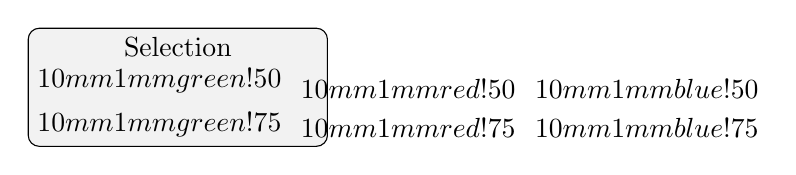
\begin{tikzpicture}
    \tikzstyle{box} = [rectangle, rounded corners, minimum width=3.8cm, minimum height=1.5cm,text centered, draw=black, fill=gray!10]

    \node [box] (selection) {};
    \node [anchor=north] at (selection.north) {Selection};

    \node (line1) [anchor=south west] at (selection.south west) {$\coloredrule{10mm}{1mm}{green!75}$};
    \node (line2) [anchor=south west] at (line1.south east) {$\coloredrule{10mm}{1mm}{red!75}$};
    \node (line3) [anchor=south west] at (line2.south east) {$\coloredrule{10mm}{1mm}{blue!75}$};
    \node (line4) [anchor=south west] at (line1.north west) {$\coloredrule{10mm}{1mm}{green!50}$};
    \node (line5) [anchor=south west] at (line2.north west) {$\coloredrule{10mm}{1mm}{red!50}$};
    \node (line6) [anchor=south west] at (line3.north west) {$\coloredrule{10mm}{1mm}{blue!50}$};

  \end{tikzpicture}
        \end{scope}

        \begin{scope}[xshift=2.5cm, yshift=-5cm]
            

\node [box] (reproduction) {};
\node [anchor=north] at (reproduction.north) {Reproduction};

\node (line1) [anchor=south west] at (reproduction.south west) {$\coloredrule{10mm}{1mm}{OliveGreen, green}$};
\node (line2) [anchor=south west] at (line1.south east) {$\coloredrule{10mm}{1mm}{red, Salmon}$};
\node (line3) [anchor=south west] at (line2.south east) {$\coloredrule{10mm}{1mm}{blue, Periwinkle}$};
\node (line4) [anchor=south west] at (line1.north west) {$\coloredrule{10mm}{1mm}{green, OliveGreen}$};
\node (line5) [anchor=south west] at (line2.north west) {$\coloredrule{10mm}{1mm}{Salmon, red}$};
\node (line6) [anchor=south west] at (line3.north west) {$\coloredrule{10mm}{1mm}{Periwinkle, blue}$};
\node (line7) [anchor=south west] at (line4.north west) {$\coloredrule{10mm}{1mm}{green}$};
\node (line8) [anchor=south west] at (line5.north west) {$\coloredrule{10mm}{1mm}{red}$};
\node (line9) [anchor=south west] at (line6.north west) {$\coloredrule{10mm}{1mm}{blue}$};
        \end{scope}

        \begin{scope}[xshift=0cm, yshift=-2.6cm]
            
  \node [box] (mutation) {};
  \node [anchor=north] at (mutation.north) {Mutation};

  % TODO: slightly shift the color of the offspring.


  \node (line1) [anchor=south west] at (mutation.south west) {$\coloredrule{10mm}{1mm}{green!75}$};
  \node (line2) [anchor=south west] at (line1.south east) {$\coloredrule{10mm}{1mm}{red!75}$};
  \node (line3) [anchor=south west] at (line2.south east) {$\coloredrule{10mm}{1mm}{blue!75}$};
  \node (line4) [anchor=south west] at (line1.north west) {$\coloredrule{10mm}{1mm}{green!50}$};
  \node (line5) [anchor=south west] at (line2.north west) {$\coloredrule{10mm}{1mm}{red!50}$};
  \node (line6) [anchor=south west] at (line3.north west) {$\coloredrule{10mm}{1mm}{blue!50}$};

        \end{scope}

        \draw[-latex, thick, shorten >=0.1cm, shorten <=0.1cm] (population) -- (phenotypes);
        \draw[-latex, thick, shorten >=0.1cm, shorten <=0.2cm] (phenotypes.east) -- (evaluation);
        \draw[-latex, thick,shorten >=0.1cm, shorten <=0.1cm] (evaluation) -- (speciate);
        \draw[-latex, thick, shorten >=0.2cm, shorten <=0.2cm] (speciate) -- (selection);
        \draw[-latex, thick, shorten >=0.2cm, shorten <=0.2cm] (selection) -- (reproduction);
        \draw[-latex, thick, shorten >=0.2cm, shorten <=0.2cm] (reproduction) -- (mutation);
        \draw[-latex, thick,shorten >=0.1cm, shorten <=0.1cm] (mutation) -- (population);

    \end{tikzpicture}
    \end{mdframed}
\end{figure}